\chapter{Preparation}\label{ch:prep}

The project builds upon an existing foundation of tools and concepts.
This chapter introduces the Elixir language used in its implementation, as well as providing a summary of concepts described in the original Dataflow paper.
The professional Software Engineering approach used throughout is also touched upon.

\section{The Elixir programming language (a primer)}\label{sec:prep:elixir}

Elixir is a modern, functional language which executes on the BEAM VM.
This section provides a short description of the language to give context for the implementation chapter.
Any special syntax or semantics in code examples will be explained where introduced.

\subsection{Language basics}\label{sec:prep:elixir:basics}

Elixir is a dynamically-typed, garbage-collected functional language.
Values are immutable and looping behaviours are implemented through recursion, making use of tail-call optimisation, as in many other functional languages.

Elixir has the usual assortment of useful data types including arbitrary-sized integers, arbitrary-sized tuples, lists, maps (dictionaries) and \emph{binaries} (which specialise to strings)~\cite[p.~23]{Thomas:2016}.

It also has \emph{atoms}, denoted \exs{:foo}.
Atoms are constant literals, with their name as their value, and can be compared very efficiently.

As such, atoms are used very often to tag tuples, for example \exs{{:ok, result}}.
These tagged tuples are very flexible and often replace the role of abstract data types in more classical functional languages.
Atoms are also often used as keys in maps~\cite[p.~29]{Thomas:2016}.

Elixir uses modules to organise functions.
A module is a namespace in which functions and macros, both public and private, can be placed~\cite[p.~58]{Thomas:2016}.
Elixir has first-class functions and supports both creating lambdas and capturing existing functions within modules as lambdas~\cite[p.~37]{Thomas:2016}.

All values in Elixir can be serialised in a standard way.
This includes functions and modules, which are serialised in their bytecode form.
That property makes it easy to send code over the wire, facilitating the distribution of work across a system.

Elixir has powerful pattern-matching capabilities, available in function heads and \exs{case} expressions~\cite[p.~13]{Thomas:2016}.
Since all values in the language can be directly expressed syntactically (there are no user-definable types), any value can be directly matched and values such as tuples, maps and lists can be destructured and their contents matched directly.
\Cref{lst:prep:pattern-matching-example} shows an example combining atoms and pattern matching.

\begin{listing}[h]
	\caption[An example Elixir module, showcasing pattern-matching.]{Elixir uses a module system to organise code. Functions in modules can have multiple heads and use pattern-matching on their arguments in order to destructure them.}
	\label{lst:prep:pattern-matching-example}
	\begin{minted}{elixir}
defmodule WidgetExample do

  @doc """
  The function `get_widget_name!` takes a widget, or a list of widgets, and returns its name
  (in the case of a list the name of the first widget is returned).

  Raises an error if the operation fails. 
  """
  # The optional @spec line documents the types accepted and returned
  # by a function, as well as improving the results of static analysis tools. 
  @spec get_widget_name!([Widget.t] | Widget.t) :: String.t
  # This function head is only executed
  # when the argument is a list with at least one element.
  def get_widget_name!([widget | _]) do
    get_widget_name!(widget)
  end
  # Maps are denoted `%{key => value}`.
  # `%Widget{}` is a special type of map, with an associated module.
  # It is called a structure.
  # `%{key: value}` is a shorthand when using atoms as map keys.
  # It is equivalent to writing `%{:key => value}`.  
  def get_widget_name!(%Widget{id: widget_id}) do
    case WidgetManager.get_name(widget_id) do
      {:ok, name} -> name
      {:error, reason} -> raise reason
    end
  end

# If the function is called with an argument that is neither a list
# nor a `%Widget{}`, a runtime match error is raised.
end
	\end{minted}
\end{listing}

Elixir has a powerful macro system, which allows for the arbitrary transformation of the Abstract Syntax Tree (AST) at compile-time~\cite[p.~13]{Elixir-Metaprogramming}.
In fact, most standard language directives such as those which define modules and functions or control program-flow are themselves macros~\cite[p.~21]{Elixir-Metaprogramming}.

Elixir programs often adopt the paradigm of data being transformed by flowing through a pipeline of functions.
To that end, the convention in Elixir for functions which operate on data is to take the value being transformed as the first argument to the function.
Then, the pipeline operator \exs{|>} is used to write expressions like
\begin{minted}[linenos=false]{elixir}
"foo"
|> String.capitalize()
|> String.pad_leading(5)
# produces "  FOO"
\end{minted}
which is equivalent to
\begin{minted}[linenos=false]{elixir}
String.pad_leading(String.capitalize("foo"), 5)		
\end{minted}
but expresses the steps in the computation much more clearly~\cite[p.~56]{Thomas:2016}.
This convention matches the Dataflow Model well, since it too works in terms of defining a pipeline of transformations for data to flow through.

\subsection{Concurrency model and the OTP framework}\label{sec:prep:elixir:otp}

Elixir and Erlang both use \emph{processes}---lightweight user-space threads managed by the VM and scheduled transparently across hardware threads~\cite[p.~185]{Thomas:2016}.
The VM can support many thousands (sometimes millions~\cite{elixir-2million-processes}) of processes with a predictable, linear performance curve (rather than a sudden drop in performance under load), making it very suitable for running highly available concurrent systems.
Processes each have their own heap and can communicate and synchronise through message-passing.
Data passed in a message is copied between process heaps, isolating their execution~\cite[p.~29]{scalability_erlang_otp}.

The OTP\footnote{
Once `Open Telecom Platform', the initialism now has no further meaning.
} framework ships with the standard Erlang distribution and provides tools to develop robust concurrent and distributed systems.
Processes are organised into supervision trees, with certain processes (\emph{supervisors}) responsible for starting, restarting, and killing child processes.
In this way crashes can be isolated and handled explicitly and locally, making for more robust and failure-tolerant systems~\cite[p.~169]{scalability_erlang_otp}.

OTP provides powerful concurrency and distribution primitives such as state machines and generic servers which handle many common edge cases and failure modes so prevalent in distributed systems.

It is a typical pattern to use these primitives to build systems with an actor model---isolated processes each handling a particular concern, communicating by sending messages.

Only a small portion of the power of OTP is used in the implementation in this project, but it has provided functionality to which thousands of lines of code are dedicated in the Beam codebase.
A full, production-ready, distributed implementation of the Model in Elixir would be able to take advantage of the advanced primitives available, greatly reducing code size and complexity and increasing performance over JVM implementations.

\section{The Dataflow Model explained}\label{sec:prep:dataflow}

This section summarises the Model as it was presented originally~\cite{Akidau:2015} in preparation for its extension (\cref{sec:impl:dataflow}) and implementation (\cref{sec:impl:approach}) in the following chapter.

The Dataflow Model is a unified model of data processing which can subsume other abstractions, placing them in a well-defined taxonomy and allowing for the efficient execution of disparate computations on one system.

It does this by decoupling the logical notion of data processing from the underlying physical implementation.
An abstract data processing model is defined which allows the orthogonal specification of \textbf{what} results are computed, \textbf{where} in event-time they are computed, \textbf{when} in processing-time they are materialised, and \textbf{how} earlier results relate to later refinements~\cite[p.~1793]{Akidau:2015}.

This standard model can then be implemented and realised by many different \emph{runners}, whether natively batch, streaming or hybrid. 
Such a runner determines its own execution strategies while producing output consistent with the Model.
This flexible approach allows for the tuning of execution technology to business requirements while working with a consistent, expressive theoretical model of the computation itself.

This model makes as few assumptions as possible about the data inputs, outputs and processes. 
Instead, it provides simple primitives from which complex systems can be constructed.

What follows is a descriptions of the primitives used in the Model to more precisely specify all of these properties.

\subsection{`The What': Transforms and Pipelines}\label{sec:prep:dataflow:what}

In the Dataflow Model, a \emph{Pipeline} is an independent computation.
It may incorporate many different \emph{Transforms} which pass data to each other, processing and transforming it as it flows through them.
One can think of Pipelines as Directed Acyclic Graphs (DAGs), with nodes representing Transforms and edges representing data flowing between them (\cref{fig:prep:pipeline-dags}).

\begin{figure}[t]
	\subfloat[][A simple Pipeline might read elements, count the number of values for each key, and save this result to a file. \texttt{ReadElements} is a Root Transform.]{
	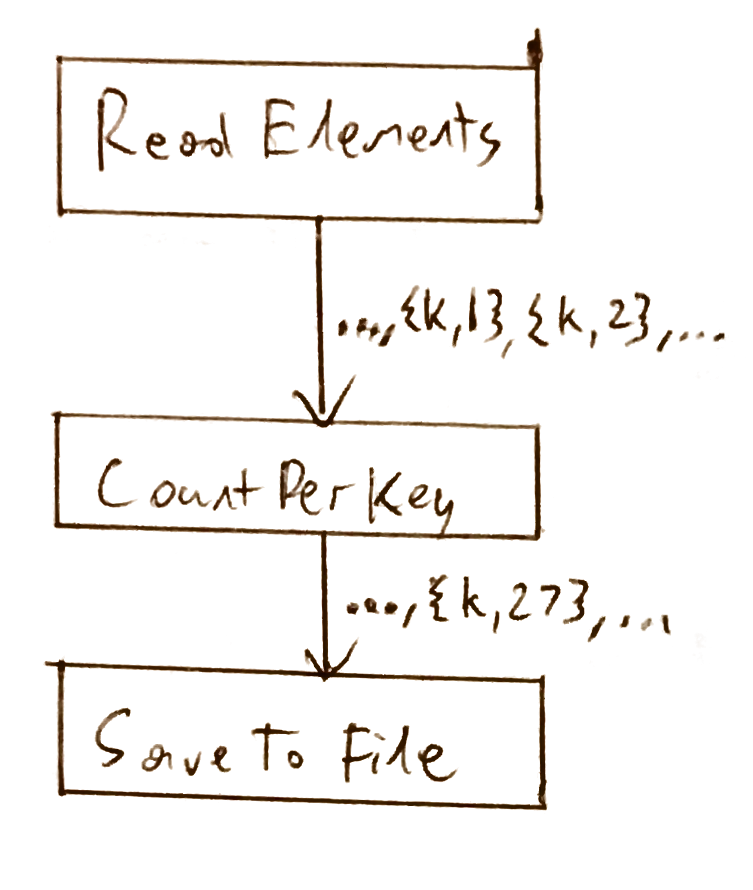
\includegraphics[width=0.3\textwidth]{images/temp/pipeline-dag-basic}
	}
	\subfloat[][A complex Pipeline can feature branching and Transforms with multiple inputs and outputs. Posts are read from a stream and partitioned into important and regular posts based on a stream of users currently considered important. \par Regular and important posts are processed in different manners, extracting information which is remerged and published to multiple external systems.]{
	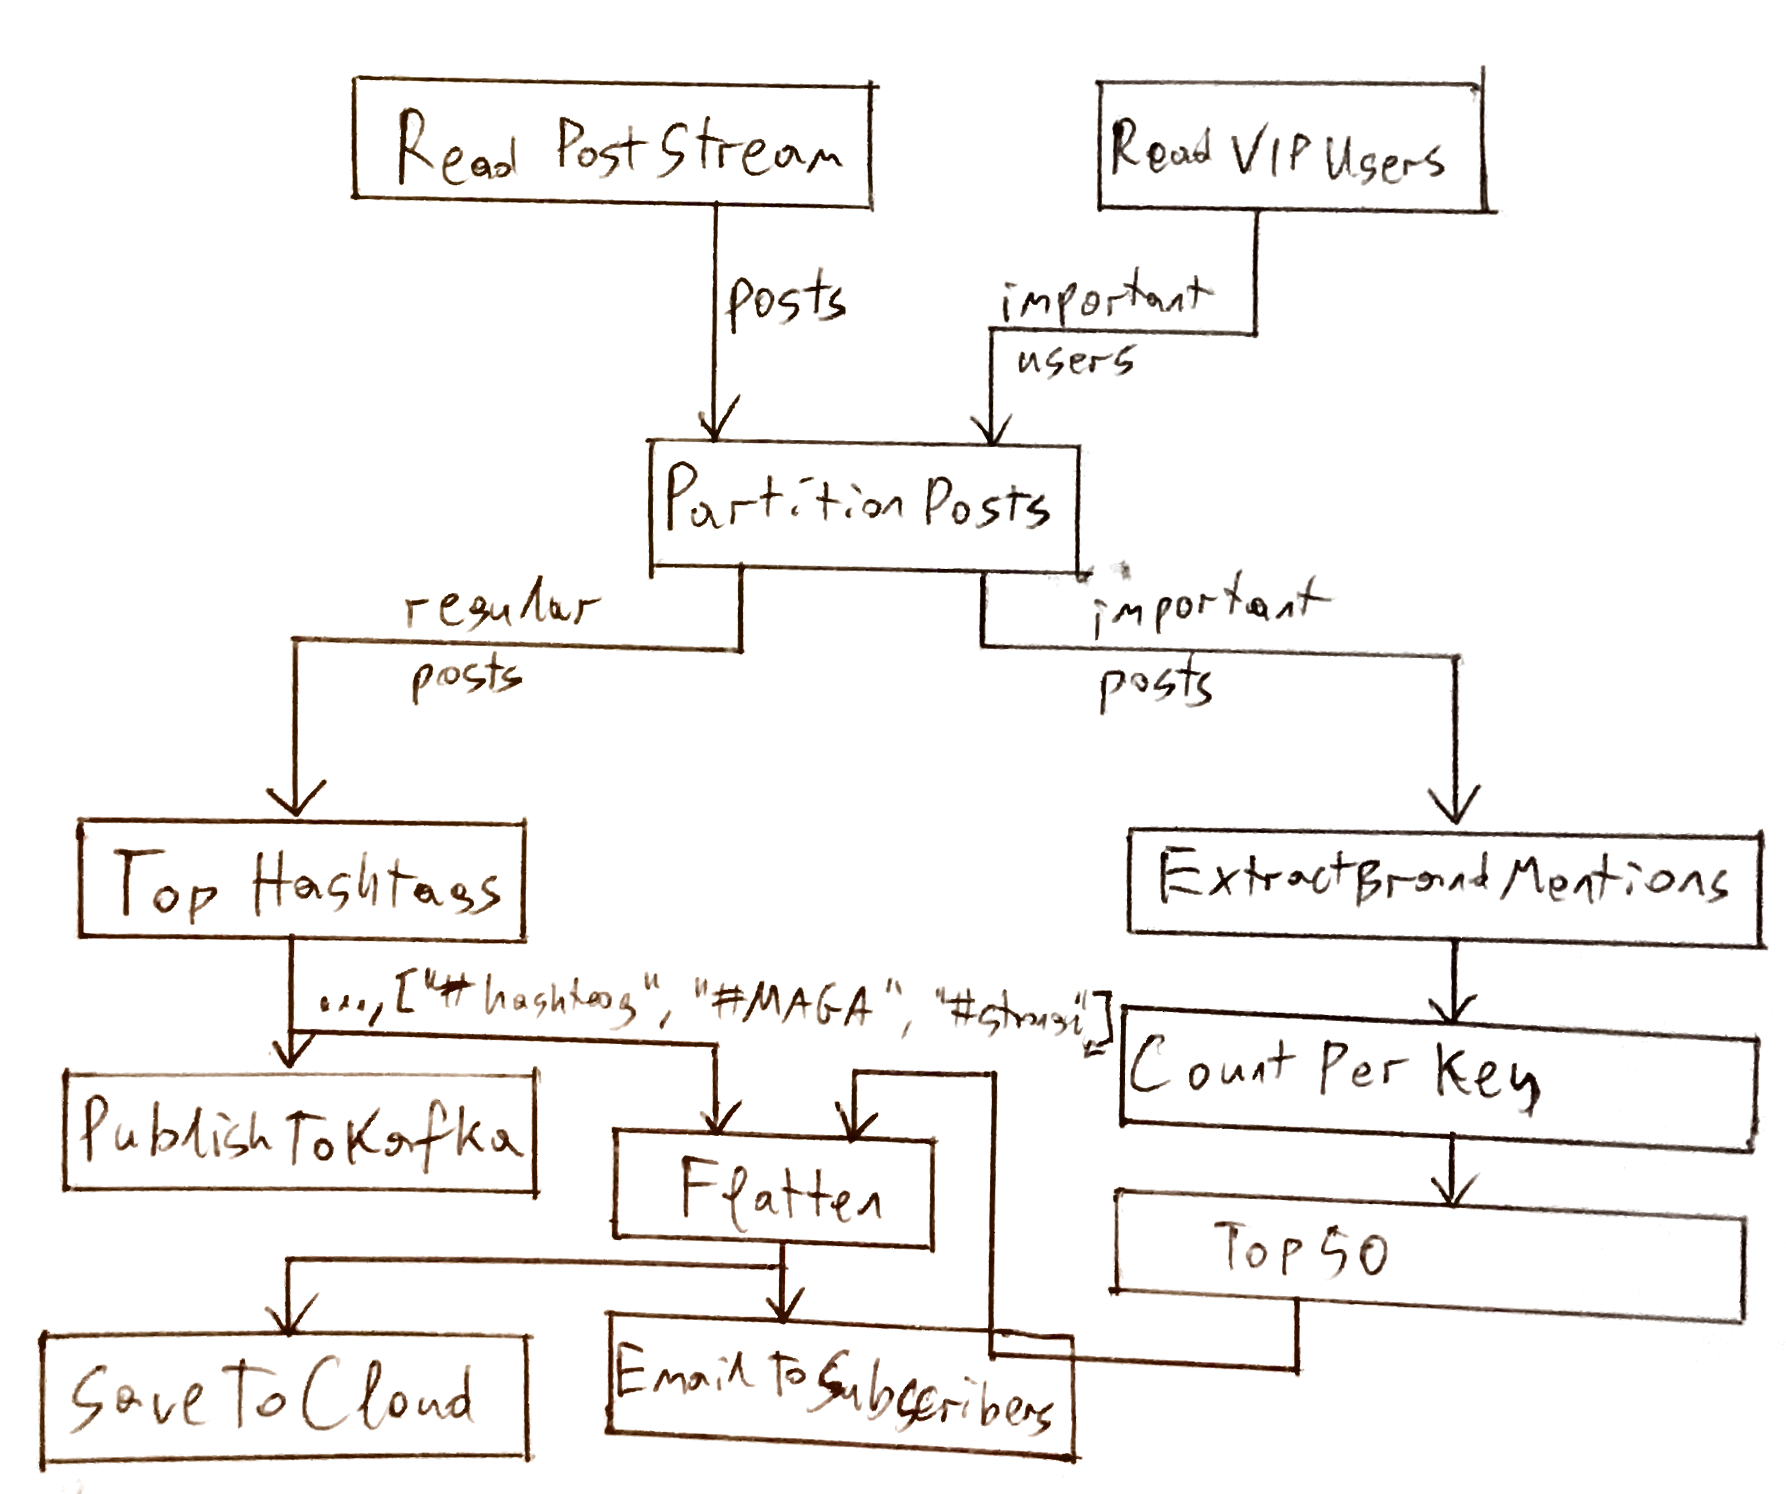
\includegraphics[width=0.7\textwidth]{images/temp/pipeline-dag-complex}
	}
	\caption[Examples of Pipelines, simple and complex, illustrated as Directed Acyclic Graphs.]{Pipelines are expressed as DAGs and can be simple or complex.}
	\label{fig:prep:pipeline-dags}
\end{figure}

A Transform may produce multiple outputs and it may consume multiple inputs.
It can also produce no outputs, instead causing a side effect such as writing to the network, database or file system.
Transforms can also have no inputs in the graph, instead receiving output from an external source or generating it.
These Transforms are called \emph{Root Transforms}.

A key advantage of expressing Transforms in terms of data flows is the natural adaptation of the system to \emph{unbounded} data streams---ones which may never finish.
An example of this may be a stream of events from a website, or the Twitter firehose.

It may help to think of unbounded data as streaming data, but `streaming' and 'batch' imply execution strategies as opposed to data properties.
Further, in the Dataflow Model it is more convenient to think of all data as streams, whether they are truly infinite or come from a file or other bounded source.

It is worth making the distinction between constructing the Pipeline by conceptually connecting Transforms and describing the computation, and actually executing the Pipeline with real data.

When the Pipeline is executed, we need to materialise the Transforms as some sort of structure which executes the processing steps declared earlier.
The data flowing at execution-time is made up of elements which can be thought of as tuples containing the data itself (often assumed to be key-value pairs), timestamps (intrinsic to the element) and any windows which have been assigned to the element (described later).

All Transforms can be represented fundamentally using only two primitives: \verb|ParDo| and \verb|GroupByKey|\footnotemark[2], illustrated in \cref{fig:prep:pardo-gbk}.

\footnotetext[2]{
Even though these Transforms are the only primitives mentioned in the original description of the Model~\cite[§2.1]{Akidau:2015}, real implementations will likely special-case several other transforms such as \texttt{AssignTimestamps} or \texttt{Window} and make them primitives for architectural or performance reasons.
}

\begin{figure}[h]
	\centering
	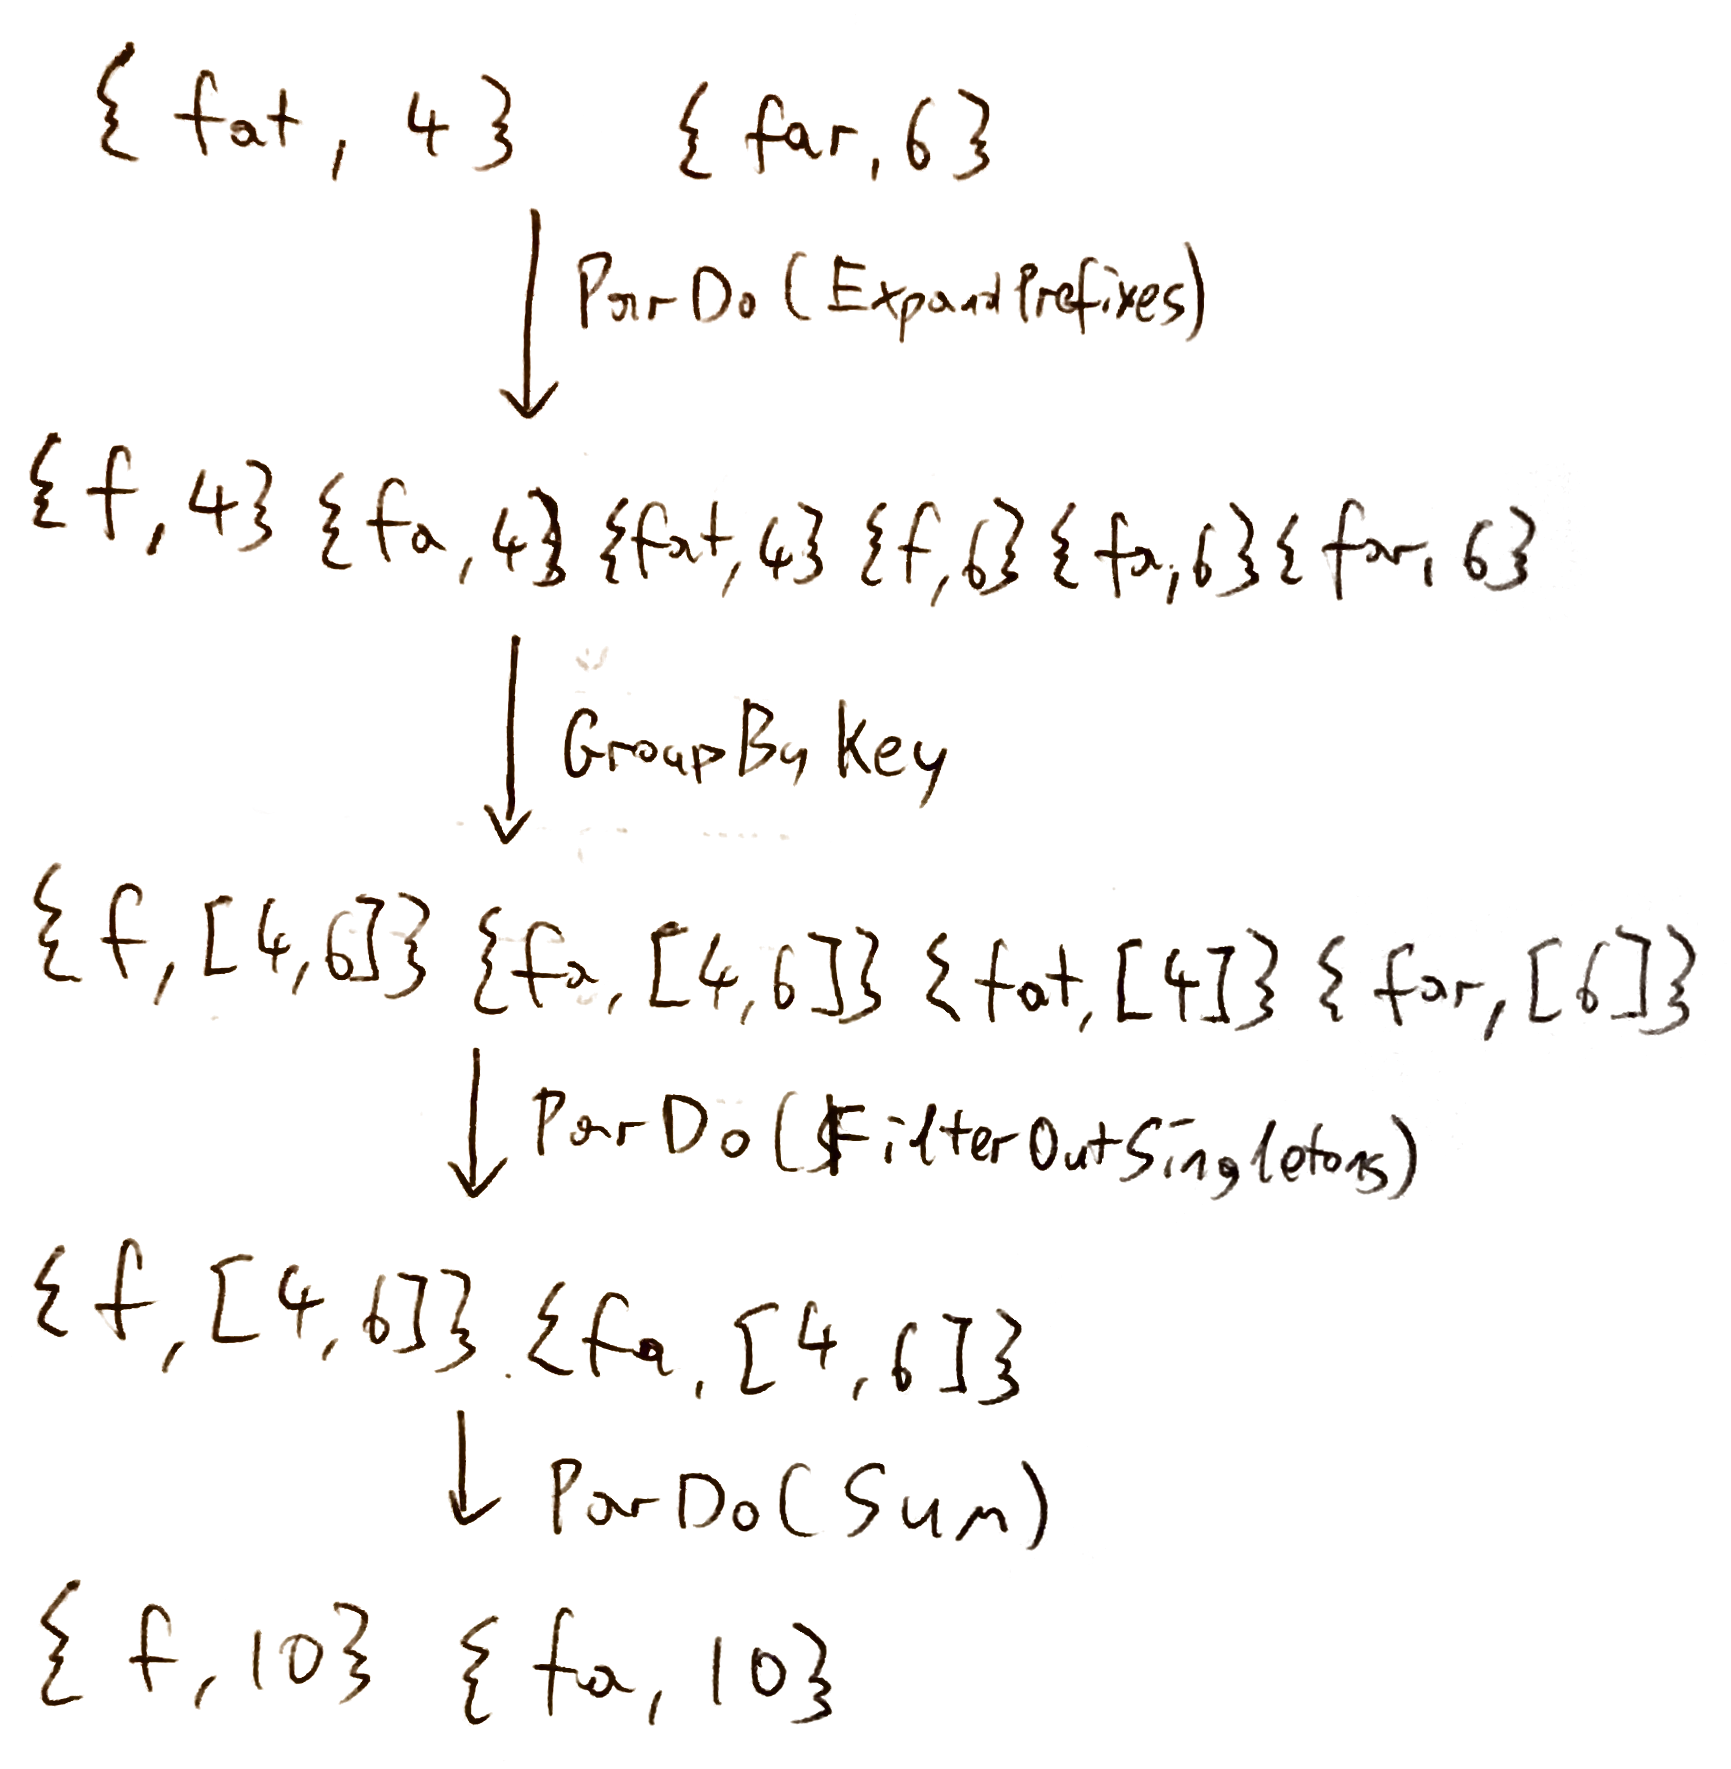
\includegraphics[width=0.6\textwidth]{images/temp/pardo-gbk}
	\label{fig:prep:pardo-gbk}
	\caption[An illustration of the operation of \texttt{ParDo} and \texttt{GroupByKey}.]{\texttt{ParDo} and \texttt{GroupByKey} are used as primitives for the construction of other Transforms. \texttt{ParDo} outputs zero or more elements per element, and \texttt{GroupByKey} outputs precisely one element per key in the input Collection.}
\end{figure}


\verb|ParDo| represents a flat-map operation---it transforms an input data element into zero or more output data elements.
Its output must depend only on the single input element.
This restriction means that the \verb|ParDo| step is embarrassingly parallelisable (with caveats, as always).
It also translates naturally to operating on unbounded data.

\verb|GroupByKey| groups all key-value pairs into per-key elements containing all values for a particular key.
It needs to collect \emph{all} of the data for a particular key before being able to emit its output.
An issue arises when dealing with unbounded data---how do we know when we have received all of the input for a particular key?

To deal with this problem, the Dataflow Model introduces windowing.

\subsection{`The Where': Windowing}\label{sec:prep:dataflow:where}

\emph{Windowing} is the additional grouping of elements according to their timestamps in a way which allows us to emit a chunk of data as soon as all relevant elements have been seen.
In the Dataflow Model, we call such a chunk of data belonging to a particular window a \emph{pane}.

Let us first formalise the notion of \emph{time} in this context before we describe the windowing process further.

\subsubsection{Time domains}

\todo{diagram?}

We distinguish between two time domains when considering our data as events in time: \emph{event-time} and \emph{processing-time}.

\emph{Event-time} describes the time in which events actually occur.
Each element in a Pipeline has an inherent timestamp in the event-time domain.
We ensure that we have two special values available, the \emph{minimal} and \emph{maximal timestamps}, representing negative and positive infinity.

Where there is no inherent time associated with an element (for example it is an un-dated record in a file) or we don't know the timestamp yet (we must process the record before we can extract the timestamp), the element is assigned the minimal timestamp.
The logic of this will become apparent in following chapters.

\emph{Processing-time} is a property of an executing Pipeline.
It measures real-world time elapsing as the computation progresses.
The processing time of an element at a Transform is the system clock time at which it was seen or processed by that Transform.

\subsubsection{Types of windows}

\begin{figure}[h]
	\subfloat[][Global windowing assigns all elements to a single, infinite window.
It is equivalent to no windowing at all.]{
		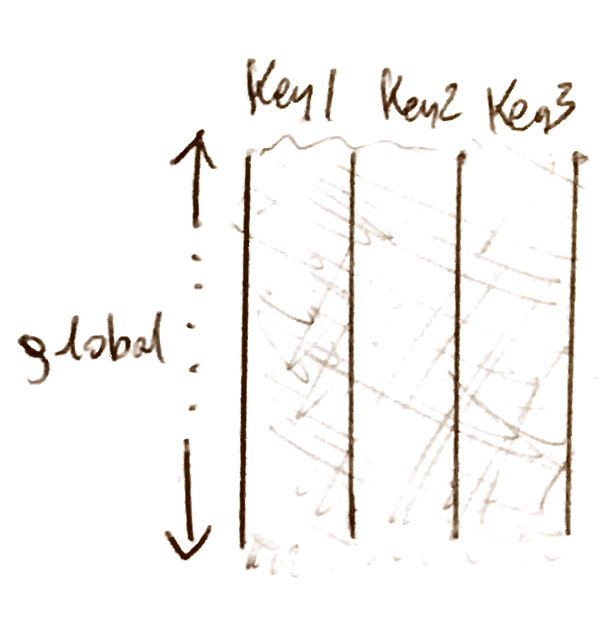
\includegraphics[width=0.5\textwidth]{images/temp/window-type-global}
	}
	\subfloat[][Fixed windows have a static window size, e.g.\ hourly, and are \emph{aligned}---each window contains all of the data in the system for that period of time.]{
		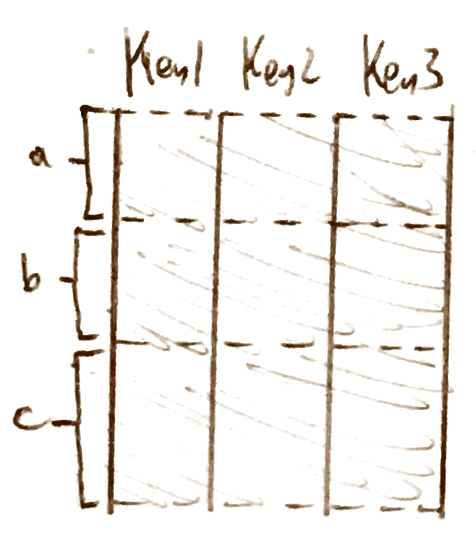
\includegraphics[width=0.5\textwidth]{images/temp/window-type-fixed}
	}\\
	\subfloat[][Sliding windows have a static window size and slide period, e.g.\ hourly windows which start every 10 minutes.
The windows may overlap, which requires the system to be able to place a single piece of data in multiple windows.
The windows are still aligned.]{
		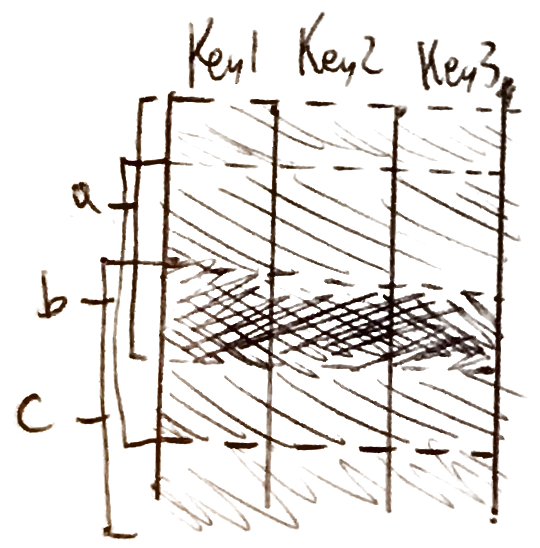
\includegraphics[width=0.5\textwidth]{images/temp/window-type-sliding}
	}
	\subfloat[][Sessions are windows which capture some period of activity over a subset of the data.
They are typically specified using a timeout after which a new session starts.
Any events closer in time than that form a session.
These windows need to be able to merge as new data is added between them.
They are also unaligned---certain windows apply only to a subset of the data.]{
		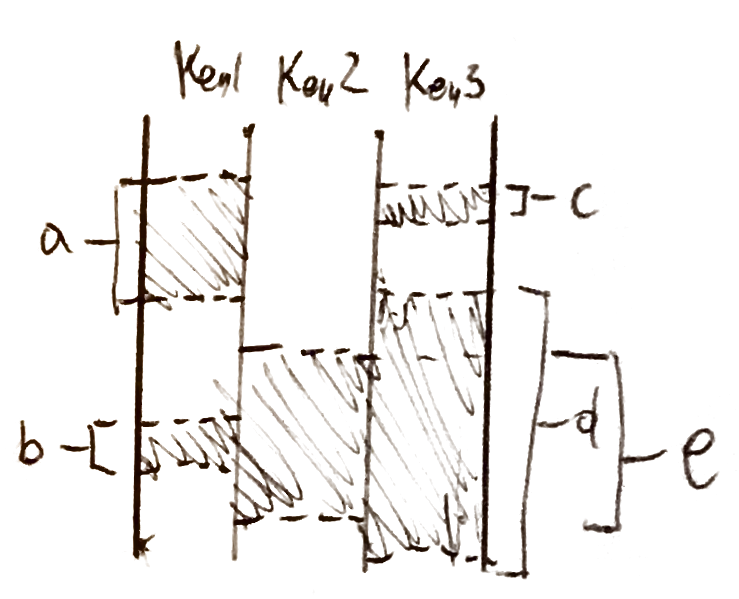
\includegraphics[width=0.5\textwidth]{images/temp/window-type-sessions}
	}
	\caption{Four windowing paradigms, all supported by the Dataflow Model.}
	\label{fig:prep:window-types}
\end{figure}

There are three windowing patterns which are commonly used in practice.
\Cref{fig:prep:window-types} describes and illustrates these, along with global windowing.

A progression in complexity is apparent, and many other systems support only a prefix of this list of paradigms.
The Dataflow Model is able to support all of these by not making assumptions about windows being aligned, non-overlapping or immutable.

\subsubsection{Windowing in the Dataflow Model}
A key part of the Dataflow Model which allows for flexible windowing is the generalisation of what a window is.
The Model requires only that a window is some deterministic, comparable value.
In practice, intervals in event-time are used.

The complexity of the different windowing paradigms is encapsulated thusly:
define a \emph{windowing function} (\verb|WindowFn|) as (somewhat counter-intuitively) a pair functions: \texttt{assign} and \texttt{merge}.

\texttt{assign} assigns a set of windows to an element.
If the element is assigned to multiple windows, the element is replicated in each of those windows (since all computation is implicitly grouped by the window).

\texttt{merge} merges some or all of an input set of windows into a new set of windows.
This is used in, for example, session windowing mentioned as earlier (illustrated in \cref{fig:prep:sessions-merge}).
Most windowing strategies do not need to merge windows.

\begin{figure}[h]
	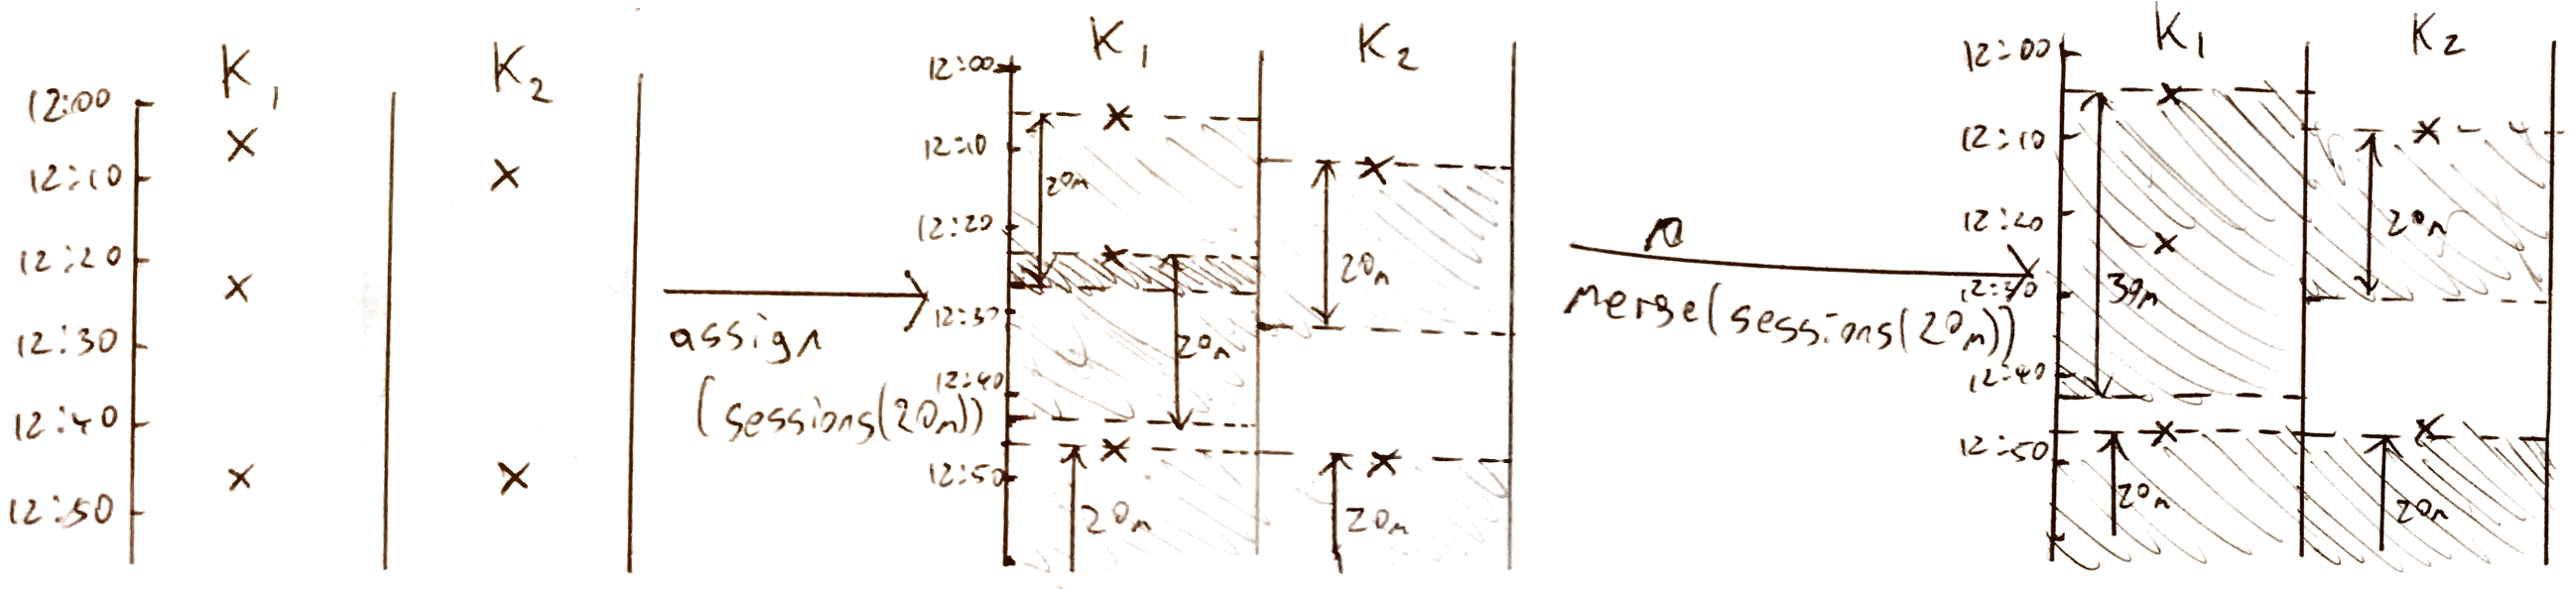
\includegraphics[width=\textwidth]{images/temp/sessions-assign-merge}
	\caption[An illustration of a \texttt{WindowFn} being used to place elements into session-based, unaligned windows.]
	{The sessions \texttt{WindowFn} is used to assign elements with two separate keys into session-based windows. The \texttt{assign} operation puts each element in each key into its own 20 minute-long window. The \texttt{merge} operation then takes any overlapping windows and merges them into a larger window spanning all original windows.}
	\label{fig:prep:sessions-merge}
\end{figure}


\subsection{`The When': Watermarks and triggers}\label{sec:prep:dataflow:when}

In the previous section, we have defined a way to group elements together into windows.
We have also asserted that we can `emit a chunk of data as soon as all relevant elements have been seen'.
How can this be achieved in light of the fact that data may appear out of order?

The true answer is that it cannot---if we allow unpredictably late data in the Pipeline, then we cannot ever truly be certain that we can emit a complete pane of data.
What we can do, however, is introduce a model which allows us to specify the desired behaviour explicitly.

Let us first define the concept of \emph{watermarks}.

\subsubsection{Watermarks}

\todo{Diagram of watermarks?}

A \emph{watermark} is a lower bound in event-time on the timestamps of values which have been processed by the Pipeline (or a particular Transform therein).
For example, if at a particular instant the watermark is $T$, then we are promised that all events with timestamps earlier than $T$ have been processed.
A graph of watermark progression against processing time (such as the one in \cref{fig:prep:watermark-progression}) is a useful way to visualise the progress of a Pipeline.
Further, this concept allows us to construct a powerful model of lateness in the system.
This is explored further in \cref{sec:impl:dataflow:lateness}.

\begin{figure}[h]
	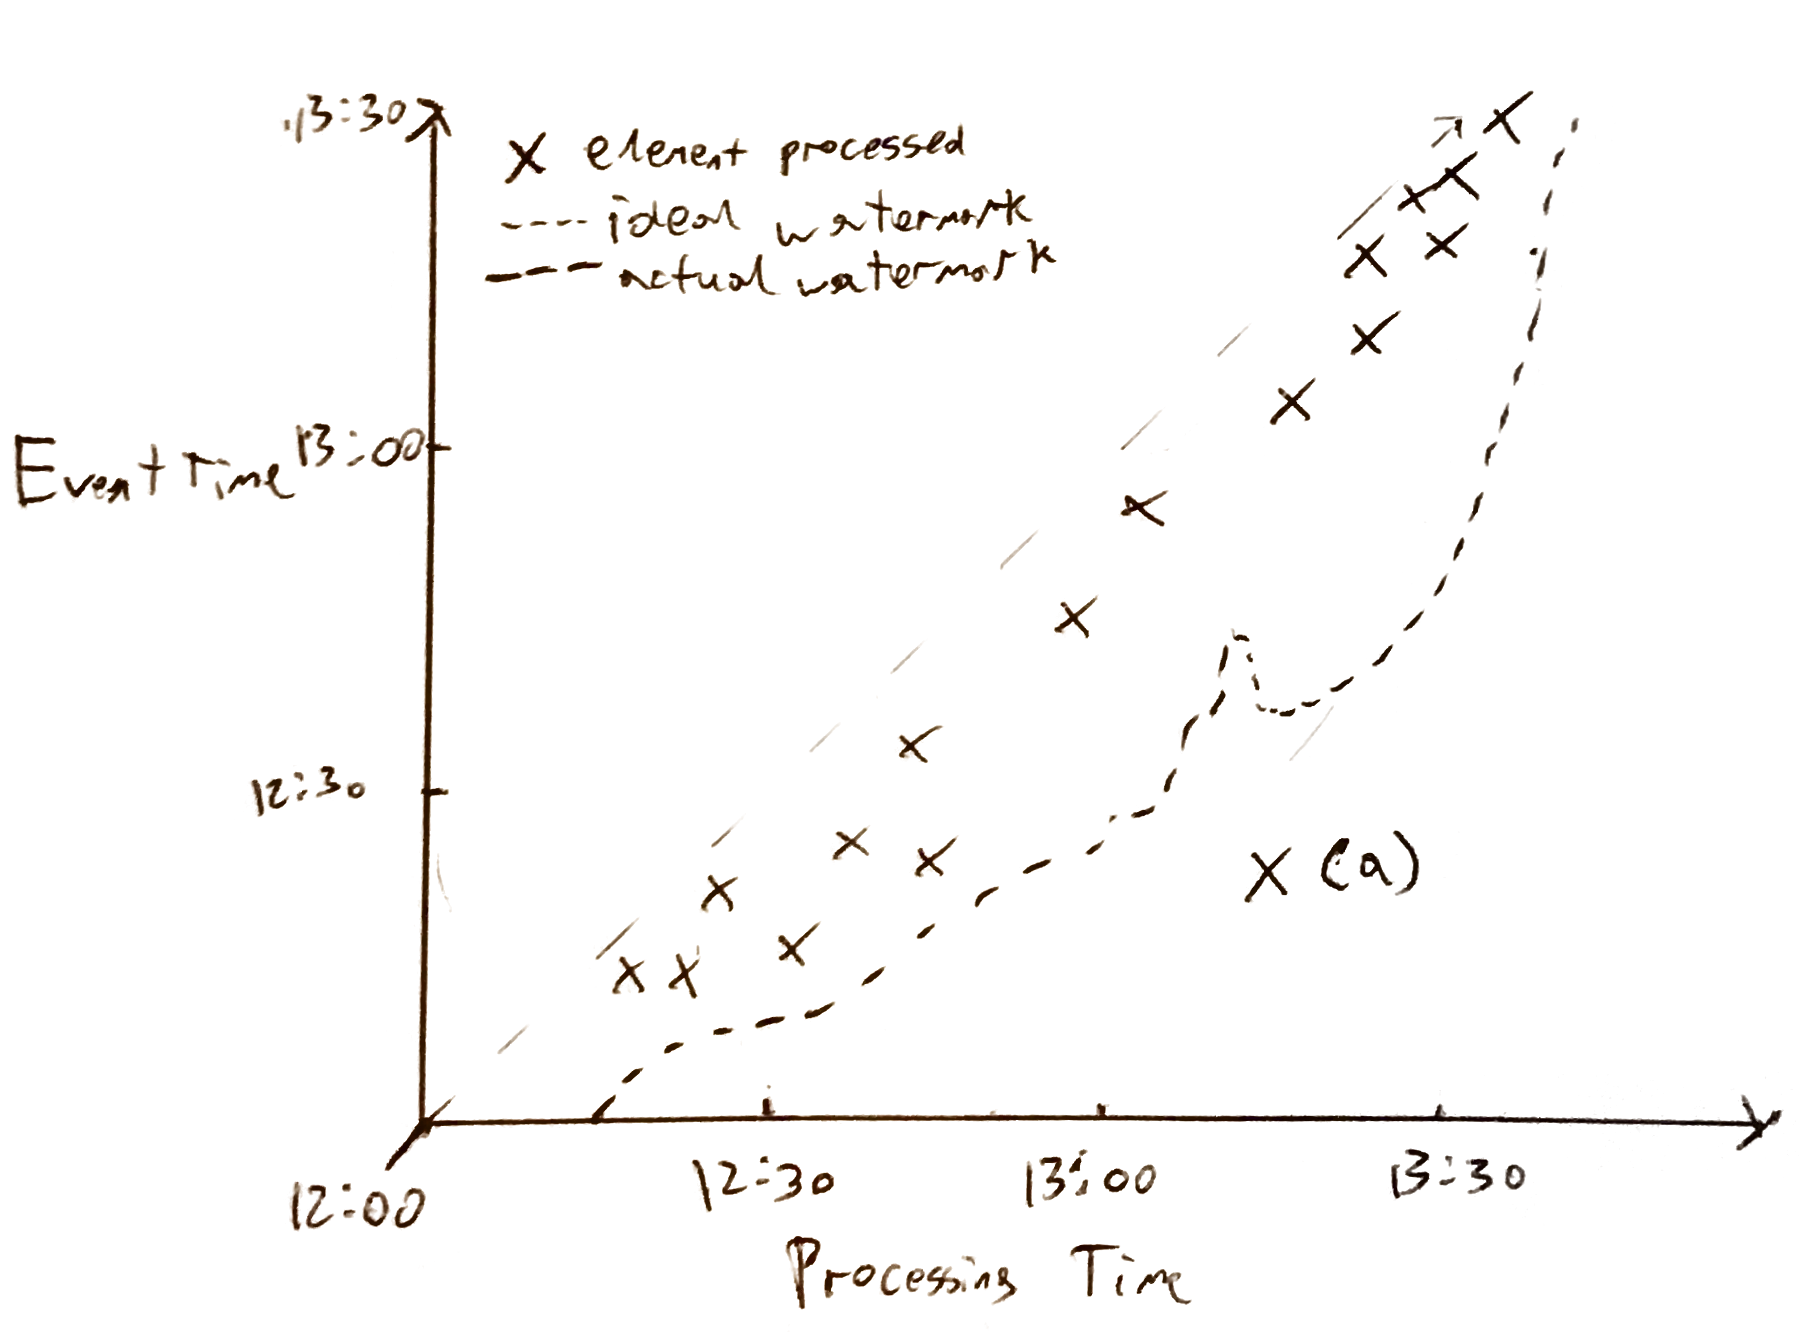
\includegraphics[width=\textwidth]{images/temp/watermark-progression-example}
	\caption[An example of a watermark progression plotted against event time, showing late data as falling behind the watermark.]{A graph of watermark progression against event time shows how up-to-date a data stream is. The ideal watermark shows the best possible result---processing each element immediately as it is produced. The actual watermark is a heuristic for the true watermark. The element marked (a) was late as it arrived behind the watermark.}
	\label{fig:prep:watermark-progression}
\end{figure}

The reader may at this point be asking, `where does the watermark come from?'
Watermarks in the Dataflow Model are heuristics generated by sources of data, or by user logic in the Pipeline.
This is described further in \cref{sec:impl:dataflow:watermark-generation}.

\subsubsection{Triggering model}

An initial suggestion may be to simply use the watermark as an indication of when a window is finished and is safe to emit; that is, to emit once the watermark has passed the end of the window.
However, it is possible for the watermark on its own to be \textbf{too fast} or \textbf{too slow}, emitting a pane too early or holding back the entire Pipeline waiting for data which may never arrive.

To solve these problems, we define a more complex triggering model.

Firstly, we explicitly allow for data in a particular window to be emitted multiple times.
We call each such emission a pane, and every pane is marked as either \verb|EARLY|, \verb|ON_TIME| or \verb|LATE|, indicating the timeliness of the data which were used to compute it.

Secondly, we define a \emph{trigger} as a Finite State Machine (FSM) which has access to time information of elements passing through the Transform, as well as watermarks and other timing information.
This FSM can instruct the Transform to emit a pane of currently buffered data at any time.

In this manner, a variety of behaviours is enabled.
For example, one may want to receive approximate results (\verb|EARLY| panes) every ten seconds (in processing-time) until the watermark passes the end of the window, at which point an \verb|ON_TIME| pane is emitted.
Any further late data arriving after the watermark can trigger the emission of a \verb|LATE| pane.

The combination of these flexible windowing and triggering models allows for a powerful, yet deterministic method of grouping and emitting data as needed, even if it is sourced from a mixture of heterogeneous, unordered, unbounded streams.
To provide these advantages, however, a considerable amount of extra machinery is required, as discussed in \crefrange{sec:impl:dataflow:windows-panes}{sec:impl:dataflow:triggers-timers}.

\subsection{`The How': Refinements and retractions}\label{sec:prep:dataflow:how}

The Model allows for the selection of a \emph{refinement mode} to be used when emitting multiple panes per window.
Each pane can either contain all of the information seen from the start of the window---the \emph{accumulating mode}, or it can only contain the information seen since the last pane was emitted---the \emph{discarding mode}.

While the Model broadly defines retractions and how they work at a high level, their implementation remains an unsolved problem and is is an area of research in the Beam project~\cite{JIRA-retractions}.
As such, this topic is out-of-scope for this project.

\section{Goals and requirements}\label{sec:prep:goals}

A side-effect of the way the Dataflow/Beam project has developed is that a large amount of development of the theory of the Model has occurred implicitly while the software was worked on.
New concepts were added \emph{in situ}, without an abstract definition.
Rather, informal proposals were written and iterated upon in code.

Therefore, the extraction of these concepts from the Java codebase into a more approachable model formed a large part of the project.
This was further necessitated by the move from OOP to a functional approach, requiring each concept to be reduced to an abstract description rather than merely transferring the class hierarchy to a new language.

The initial project plan did not account for this---it was assumed that a reasonable implementation could be produced from the Dataflow paper~\cite{Akidau:2015} using the Beam code simply as reference.

\section{Software Engineering methods}\label{sec:prep:softeng}

The interleaving of research and engineering required a particular approach to the execution of the project in order to keep the project on-track and enable success.

\subsection{The spiral model}\label{sec:prep:softeng:spiral}

The fluid goals of the implementation resulted in a need for an adaptive and agile development process, since fundamental assumptions made initially changed many times over.
Often, core modules had to be re\"implemented as the model being extracted grew more complete.

The Elixir language, with its modular structure and a convention of writing simple, composable functions enabled a flexible model where key logic in the codebase could be refactored with ease when needed.

A spiral model~\cite{Boehm:1986} of development was adopted with core modules prototyped, integrated, and then refactored, extended or rewritten as other parts of the system demanded it.
The process is illustrated in \cref{fig:prep:spiral-model}.

Overall, three or four iterations of prototyping and evaluating were performed, going from a basic proof-of-concept to a working system implementing many key features of the Model.

\begin{figure}[h]
	\centering
	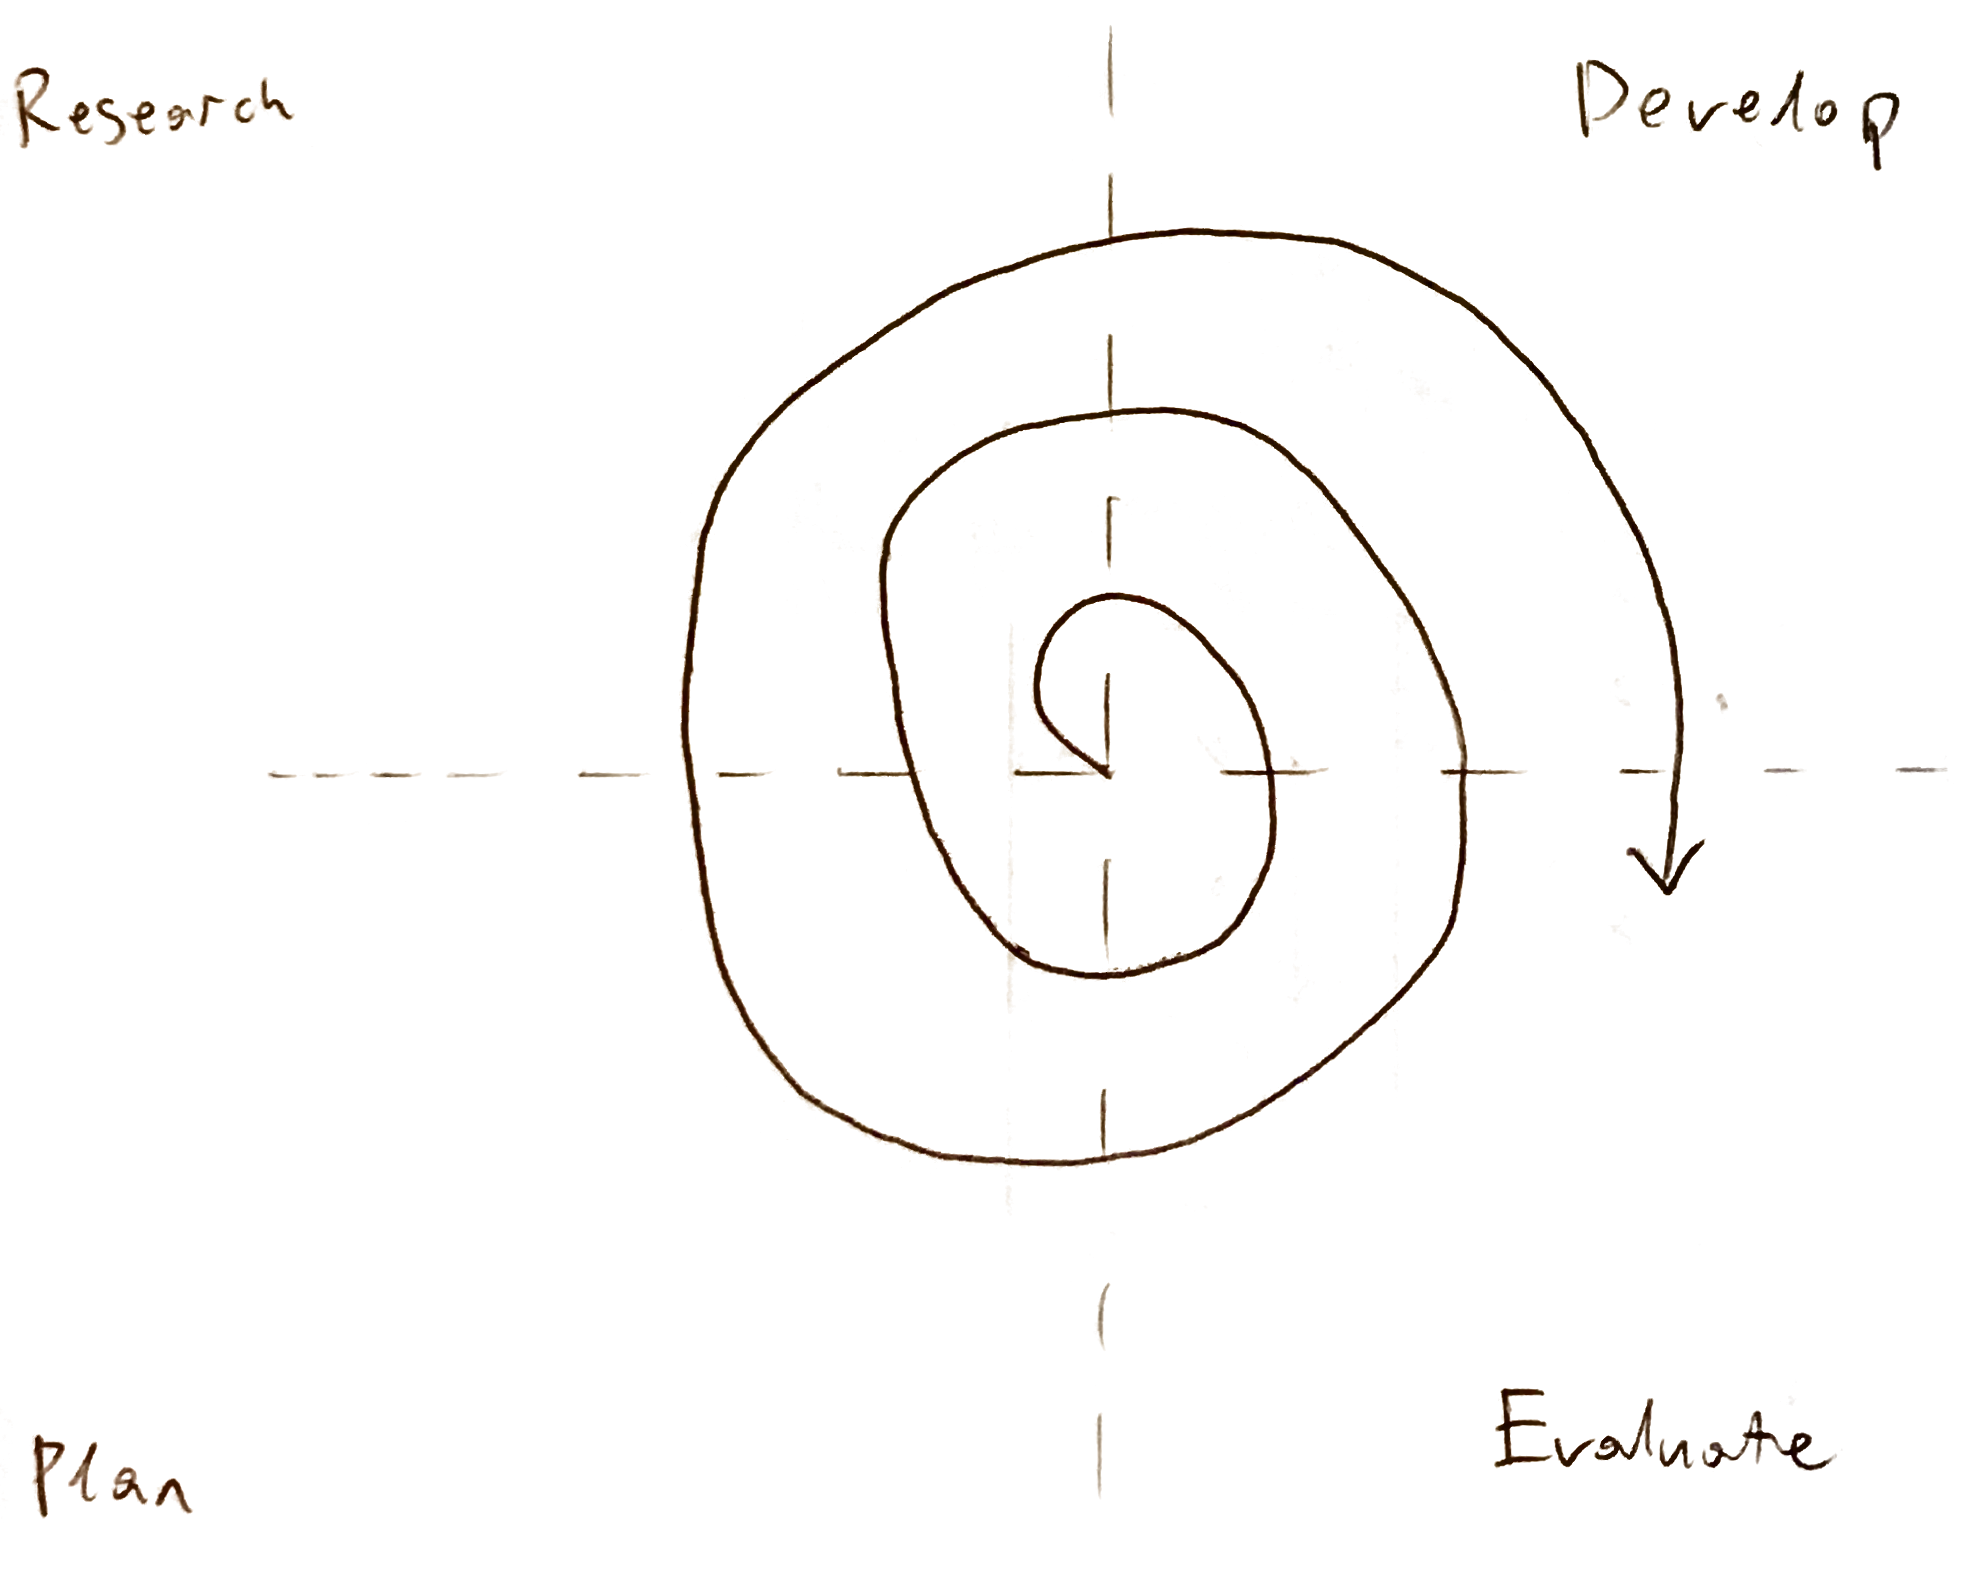
\includegraphics[width=0.6\textwidth]{images/temp/spiral}
	\caption{The spiral model of development as used in this project.}
	\label{fig:prep:spiral-model}
\end{figure}


\todo{Flesh the diagram out more, indicate the features completed at each prototype iteration.}

\subsection{Source code management}\label{sec:prep:softeng:scm}

The project source code was managed using Git, including a private GitHub upstream repository.

Source control was used to checkpoint and document progress.
This made it easy and safe to `move fast and break things', which is very useful in a prototyping-driven project.

The dissertation sources were also kept in Git, with all project data being synced to Dropbox as well as an external backup service to guard against data loss.

\subsection{Testing approach}\label{sec:prep:softeng:testing}

Owing to the modular nature of Elixir making it easy to write small modules with pure functions, module-level unit testing was employed.
Small tests were written in order to check the invariants required by the model were satisfied by the implementation.

Additionally, several end-to-end examples were written to exercise the entire system.
Some of these were also re\"implemented in Java and used for comparison purposes in the evaluation phase of the project.

\section{Starting point}\label{sec:prep:starting}

The project was started from scratch---all core code in the implementation was written specifically for this project, during the timeframe of the project.
The author had a good working knowledge of Elixir, having had implemented several projects in it before, but had no experience working with Dataflow or Beam.

The open-source Beam project was used as a reference, but due to fundamental paradigm differences the dissertation project did not simply comprise the transfer of the OOP hierarchy of the system from one language to another.